\documentclass[11pt]{article}

% Essential packages
\usepackage[utf8]{inputenc}
\usepackage[T1]{fontenc}
\usepackage{amsmath, amssymb, amsthm}
\usepackage{mathtools}
\usepackage{algorithm}
\usepackage{algorithmic}
\usepackage{listings}
\usepackage{xcolor}
\usepackage{tikz}
\usetikzlibrary{arrows.meta, positioning}
\usepackage{hyperref}
\usepackage[margin=1in]{geometry}

% Theorem environments
\newtheorem{theorem}{Theorem}[section]
\newtheorem{lemma}[theorem]{Lemma}
\newtheorem{proposition}[theorem]{Proposition}
\newtheorem{corollary}[theorem]{Corollary}
\theoremstyle{definition}
\newtheorem{definition}[theorem]{Definition}
\newtheorem{example}[theorem]{Example}

% Custom commands
\newcommand{\R}{\mathbb{R}}
\newcommand{\E}{\mathbb{E}}
\newcommand{\N}{\mathcal{N}}
\newcommand{\grad}{\nabla}
\newcommand{\divergence}{\text{div}\,}
\renewcommand{\Pr}{\mathbb{P}}
\DeclareMathOperator*{\argmin}{arg\,min}
\DeclareMathOperator*{\argmax}{arg\,max}

% Code listing style
\lstdefinestyle{py}{
    language=Python,
    basicstyle=\ttfamily\small,
    keywordstyle=\color{blue}\bfseries,
    commentstyle=\color{gray}\itshape,
    stringstyle=\color{red},
    showstringspaces=false,
    breaklines=true,
    frame=single,
    numbers=left,
    numberstyle=\tiny\color{gray},
    captionpos=b,
    tabsize=2
}

\title{Score Matching and Noise Conditional Score Networks:\\
A Comprehensive Lecture Note with Derivations and Code}
\author{Your Name}
\date{\today}

\begin{document}
\maketitle

\begin{abstract}
This note provides a comprehensive treatment of score matching and score-based generative modeling, 
developing the theory from first principles through modern applications. 
We begin with the fundamental score matching objective of Hyv\"arinen (2005), 
establish its connection to Fisher divergence, and proceed through denoising score matching (Vincent, 2011), 
sliced score matching (Song \& Ermon, 2019), and noise conditional score networks (Song \& Ermon, 2019, 2020). 
We connect these methods to the broader landscape of diffusion models (Sohl-Dickstein et al., 2015; Ho et al., 2020) 
and reverse-time SDEs, while maintaining rigorous derivations and practical Python implementations on two-dimensional datasets. 
The goal is pedagogical: to provide graduate students and researchers with both mathematical depth and computational intuition 
for these foundational techniques in modern generative modeling.
\end{abstract}

\tableofcontents

\section{Introduction and Motivation}

\subsection{The energy-based modeling problem}
Probabilistic modeling seeks to learn a density $p(x)$ over data $x \in \mathbb{R}^d$. 
Energy-based models (EBMs) represent this density through an energy function:
\begin{equation}
p_\theta(x) = \frac{1}{Z_\theta} \exp(-E_\theta(x)),
\quad \text{where} \quad
Z_\theta = \int_{\mathbb{R}^d} \exp(-E_\theta(x))\,dx.
\end{equation}
The partition function $Z_\theta$ is typically intractable to compute or differentiate, 
making maximum likelihood estimation challenging. 
The gradient of the log-likelihood with respect to parameters is:
\begin{equation}
\nabla_\theta \log p_\theta(x) = -\nabla_\theta E_\theta(x) - \nabla_\theta \log Z_\theta,
\end{equation}
where the second term requires sampling from the current model or expensive importance weighting.

\subsection{The score function and its properties}
The \emph{score function} is defined as the gradient of the log-density:
\begin{equation}
s(x) \coloneqq \nabla_x \log p(x).
\end{equation}
For an energy-based model, the score has a remarkable property:
\begin{equation}
s_\theta(x) = \nabla_x \log p_\theta(x) = -\nabla_x E_\theta(x) - \nabla_x \log Z_\theta = -\nabla_x E_\theta(x),
\end{equation}
because the partition function is independent of $x$. 
This eliminates the intractable normalization constant from the objective, 
forming the basis of score matching.

\subsection{Geometric interpretation}
The score function $s(x)$ is a vector field that points in the direction of steepest ascent of $\log p(x)$. 
In high-density regions, the score points toward the mode; 
in low-density regions, it points toward nearby high-density areas. 
This geometric perspective motivates sampling algorithms that follow the score field.

\section{Score Matching: Theory and Derivation}

\subsection{Fisher divergence and the score matching objective}
Let $p_{\text{data}}$ denote the true data distribution and $p_\theta$ the model. 
The \emph{Fisher divergence} measures the expected squared distance between score functions:
\begin{equation}
\label{eq:fisher}
D_F(p_{\text{data}}\,\Vert\,p_\theta)
= \frac{1}{2}\mathbb{E}_{x \sim p_{\text{data}}} \left[ \left\| \nabla_x \log p_\theta(x) - \nabla_x \log p_{\text{data}}(x) \right\|^2 \right].
\end{equation}
Expanding the squared norm and dropping the constant term $\mathbb{E}[\|\nabla_x \log p_{\text{data}}(x)\|^2]$, we obtain:
\begin{equation}
\label{eq:fisher-expanded}
J(\theta) = \mathbb{E}_{x\sim p_{\text{data}}}\left[ \frac{1}{2} \| s_\theta(x) \|^2 - s_\theta(x)^\top \nabla_x \log p_{\text{data}}(x) \right],
\end{equation}
where $s_\theta(x) = \nabla_x \log p_\theta(x)$ is the model score.

\subsection{Integration by parts: Hyv\"arinen's key insight}
The challenge is that the second term in \eqref{eq:fisher-expanded} requires access to $\nabla_x \log p_{\text{data}}(x)$, which is unknown. 
Hyv\"arinen's key contribution was showing this term can be rewritten using only $p_{\text{data}}(x)$ and $s_\theta(x)$.

\begin{theorem}[Hyv\"arinen 2005]
Under regularity conditions (differentiability, $\mathbb{E}_{p_{\text{data}}}[\|s_\theta(x)\|^2]<\infty$, and 
$\lim_{\|x\|\to\infty}p_{\text{data}}(x)s_{\theta,i}(x)=0$ for all $i$), we have:
\begin{equation}
\mathbb{E}_{p_{\text{data}}}[s_\theta(x)^\top \nabla_x \log p_{\text{data}}(x)] 
= -\mathbb{E}_{p_{\text{data}}}[\text{tr}(\nabla_x s_\theta(x))],
\end{equation}
where $\text{tr}(\nabla_x s_\theta(x)) = \sum_{i=1}^d \frac{\partial s_{\theta,i}(x)}{\partial x_i}$ is the divergence of the score field.
\end{theorem}

\begin{proof}
For each component $i$:
\begin{align}
\mathbb{E}_{p_{\text{data}}}[s_{\theta,i}(x) \cdot \partial_i \log p_{\text{data}}(x)]
&= \int p_{\text{data}}(x) \cdot s_{\theta,i}(x) \cdot \frac{\partial_i p_{\text{data}}(x)}{p_{\text{data}}(x)} dx \nonumber\\
&= \int s_{\theta,i}(x) \cdot \partial_i p_{\text{data}}(x) \, dx \nonumber\\
&= \underbrace{\left[s_{\theta,i}(x) p_{\text{data}}(x)\right]_{\partial\mathbb{R}^d}}_{=0 \text{ by boundary condition}}
- \int p_{\text{data}}(x) \cdot \partial_i s_{\theta,i}(x) \, dx \nonumber\\
&= -\mathbb{E}_{p_{\text{data}}}[\partial_i s_{\theta,i}(x)].
\end{align}
Summing over all dimensions gives the result.
\end{proof}

This yields the canonical \emph{score matching objective}:
\begin{equation}
\label{eq:score-matching}
\boxed{
\mathcal{J}_{\text{SM}}(\theta)
= \mathbb{E}_{x\sim p_{\text{data}}}\left[\frac{1}{2} \|s_\theta(x)\|^2 + \text{tr}(\nabla_x s_\theta(x))\right]
}
\end{equation}

\subsection{Computational implementation}
The divergence term requires computing $\sum_{i=1}^d \frac{\partial s_{\theta,i}}{\partial x_i}$, 
which involves $d$ backward passes through the network. 
Below is the implementation using PyTorch's autograd:

\begin{lstlisting}[style=py,caption={Exact score matching with Jacobian computation}]
def jacobian(f, x):
    """Compute full Jacobian matrix of f at x."""
    B, N = x.shape
    y = f(x)
    jac = []
    for i in range(N):
        v = torch.zeros_like(y)
        v[:, i] = 1.
        dy_i_dx = autograd.grad(
            y, x, grad_outputs=v,
            retain_graph=True, create_graph=True
        )[0]
        jac.append(dy_i_dx)
    return torch.stack(jac, dim=2).requires_grad_()

def score_matching(model, samples):
    """Hyvarinen's score matching objective."""
    samples.requires_grad_(True)
    s = model(samples)
    norm_loss = torch.norm(s, dim=-1)**2 / 2.
    J = jacobian(model, samples)
    trace_loss = torch.diagonal(J, dim1=-2, dim2=-1).sum(-1)
    return (norm_loss + trace_loss).mean()
\end{lstlisting}

\section{Challenges and Limitations}

\subsection{The manifold hypothesis}
\textbf{Problem:} Real high-dimensional data often concentrate on or near low-dimensional manifolds. 
For example, natural images occupy a tiny fraction of pixel space. 
When $p_{\text{data}}$ is supported on a manifold $\mathcal{M} \subset \mathbb{R}^d$ with $\dim(\mathcal{M}) < d$, 
the score $\nabla_x \log p_{\text{data}}(x)$ is undefined in the normal directions to $\mathcal{M}$.

\textbf{Consequence:} Classical score matching can be inconsistent—the learned score may not converge to the true score even with infinite data and capacity.

\subsection{Low-density regions and numerical instability}
\textbf{Problem:} When $p_{\text{data}}(x) \approx 0$, the log-density $\log p_{\text{data}}(x) \to -\infty$, 
and its gradient becomes ill-defined or numerically unstable.

\textbf{Consequence:} 
\begin{enumerate}
\item Training instability: Score estimates have high variance in low-density regions.
\item Sampling difficulty: Langevin dynamics initialized in low-density regions may never reach high-density areas, as the score provides weak guidance.
\end{enumerate}

These fundamental limitations motivated the development of denoising and noise-conditional approaches.

\section{Denoising Score Matching}

\subsection{The noise perturbation strategy}
Vincent (2011) proposed adding small Gaussian noise to address both manifold and low-density issues:
\begin{equation}
\tilde{x} = x + \sigma \epsilon, \quad \text{where } x \sim p_{\text{data}}, \; \epsilon \sim \mathcal{N}(0, I).
\end{equation}
The perturbed distribution is:
\begin{equation}
q_\sigma(\tilde{x}) = \int p_{\text{data}}(x) \, \mathcal{N}(\tilde{x} \mid x, \sigma^2 I) \, dx.
\end{equation}
Key properties:
\begin{itemize}
\item $q_\sigma$ has full support on $\mathbb{R}^d$, resolving the manifold issue.
\item $q_\sigma(\tilde{x}) > 0$ everywhere, stabilizing score estimation.
\item As $\sigma \to 0$, we have $q_\sigma \to p_{\text{data}}$ (in suitable topology).
\end{itemize}

\subsection{The denoising objective}
\textbf{Denoising Score Matching (DSM)} minimizes:
\begin{equation}
\label{eq:dsm}
\mathcal{J}_{\text{DSM}}(\theta; \sigma)
= \mathbb{E}_{x\sim p_{\text{data}}}\mathbb{E}_{\tilde{x}\sim \mathcal{N}(x,\sigma^2 I)}
\left[\frac{1}{2} \left\| s_\theta(\tilde{x}) - \nabla_{\tilde{x}}\log q_\sigma(\tilde{x}\mid x)\right\|^2\right].
\end{equation}
The conditional score has a simple closed form:
\begin{equation}
\nabla_{\tilde{x}}\log q_\sigma(\tilde{x}\mid x) = \nabla_{\tilde{x}}\log \mathcal{N}(\tilde{x}\mid x,\sigma^2 I) = -\frac{\tilde{x} - x}{\sigma^2}.
\end{equation}
Therefore, the target is directly computable from data samples.

\subsection{Vincent's equivalence theorem}
Vincent proved three key results:

\begin{theorem}[Vincent 2011]
The following three objectives are equivalent up to constants:
\begin{enumerate}
\item \textbf{Explicit score matching on $q_\sigma$:}
\[
\mathbb{E}_{\tilde{x} \sim q_\sigma}\left[\frac{1}{2}\|s_\theta(\tilde{x})\|^2 - s_\theta(\tilde{x})^\top \nabla_{\tilde{x}} \log q_\sigma(\tilde{x})\right]
\]
\item \textbf{Implicit score matching on $q_\sigma$:}
\[
\mathbb{E}_{\tilde{x} \sim q_\sigma}\left[\frac{1}{2}\|s_\theta(\tilde{x})\|^2 + \text{tr}(\nabla_{\tilde{x}} s_\theta(\tilde{x}))\right]
\]
\item \textbf{Denoising score matching:}
\[
\mathbb{E}_{x\sim p_{\text{data}}}\mathbb{E}_{\epsilon}\left[\frac{1}{2}\left\|s_\theta(x+\sigma\epsilon) + \frac{x+\sigma\epsilon - x}{\sigma^2}\right\|^2\right]
\]
\end{enumerate}
\end{theorem}

\textbf{Implications:}
\begin{itemize}
\item DSM implicitly performs score matching on the smoothed density $q_\sigma$.
\item The equivalence to denoising autoencoder (DAE) reconstruction shows that DAEs learn score functions.
\item We can train on easily accessible perturbed samples without computing Jacobians.
\end{itemize}

\subsection{Implementation}
\begin{lstlisting}[style=py,caption={Denoising score matching loss}]
def denoising_score_matching(scorenet, samples, sigma=0.01):
    """Vincent's denoising score matching."""
    noise = torch.randn_like(samples) * sigma
    x_tilde = samples + noise
    # Target score: -noise/sigma^2 = -(x_tilde - x)/sigma^2
    target = -noise / (sigma**2)
    scores = scorenet(x_tilde)
    scores = scores.view(scores.shape[0], -1)
    target = target.view(target.shape[0], -1)
    return 0.5 * ((scores - target)**2).sum(dim=-1).mean()
\end{lstlisting}

\subsection{Choosing the noise level}
The choice of $\sigma$ involves a trade-off:
\begin{itemize}
\item \textbf{Small $\sigma$:} Better approximation of $p_{\text{data}}$, but manifold/low-density issues persist.
\item \textbf{Large $\sigma$:} Stable training and full support, but over-smoothing loses fine structure.
\end{itemize}
This tension motivates multi-scale approaches.

\section{Sliced Score Matching}

\subsection{Motivation: computational efficiency}
The divergence term $\text{tr}(\nabla_x s_\theta(x))$ requires computing all $d$ diagonal entries of the Jacobian, 
scaling as $O(d^2)$ or $O(d)$ backward passes. 
For high-dimensional problems, this becomes prohibitive.

\subsection{Hutchinson's trace estimator}
For any matrix $A \in \mathbb{R}^{d \times d}$:
\begin{equation}
\text{tr}(A) = \mathbb{E}_{v \sim \mathcal{N}(0,I)}[v^\top A v],
\end{equation}
where the expectation is over random Gaussian vectors. 
This reduces trace computation to a single matrix-vector product.

\subsection{Sliced score matching objective}
Song \& Ermon (2019) applied this to score matching:
\begin{equation}
\label{eq:ssm}
\boxed{
\mathcal{J}_{\text{SSM}}(\theta)
= \mathbb{E}_{x \sim p_{\text{data}}} \mathbb{E}_{v \sim \mathcal{N}(0,I)}\left[\frac{1}{2} \|s_\theta(x)\|^2 + v^\top \nabla_x s_\theta(x) \, v\right]
}
\end{equation}
The term $v^\top \nabla_x s_\theta(x) \, v$ is a Jacobian-vector product (JVP), 
computable via forward-mode automatic differentiation in a single pass.

\subsection{Properties and advantages}
\begin{itemize}
\item \textbf{Computational cost:} $O(d)$ instead of $O(d^2)$, enabling scaling to high dimensions.
\item \textbf{Variance:} Single-sample Monte Carlo estimator; can use multiple projections to reduce variance.
\item \textbf{Consistency:} Under the same regularity conditions as standard score matching.
\end{itemize}

\subsection{Implementation}
\begin{lstlisting}[style=py,caption={Sliced score matching with Hutchinson estimator}]
def sliced_score_matching(model, samples, n_particles=1):
    """Sliced score matching with random projections."""
    samples.requires_grad_(True)
    loss = 0.
    for _ in range(n_particles):
        v = torch.randn_like(samples)
        # Compute score and Jacobian-vector product
        s, jvp = autograd.functional.jvp(
            model, samples, v, create_graph=True
        )
        # Score norm term
        loss += (s * s).sum(-1) / 2.
        # Trace estimator: v^T J v
        loss += (jvp * v).sum(-1)
    return (loss / n_particles).mean()
\end{lstlisting}

\section{Noise Conditional Score Networks (NCSNs)}

\subsection{The multi-scale approach}
Neither a single small $\sigma$ nor a single large $\sigma$ is ideal. 
Song \& Ermon (2019, 2020) proposed training a single conditional model across a geometric sequence of noise levels:
\begin{equation}
\sigma_1 > \sigma_2 > \cdots > \sigma_K, \quad \text{e.g., } \sigma_k = \sigma_{\max} \cdot \left(\frac{\sigma_{\min}}{\sigma_{\max}}\right)^{(k-1)/(K-1)}.
\end{equation}

\subsection{Annealed denoising score matching}
The training objective aggregates DSM losses over all noise scales:
\begin{equation}
\label{eq:ncsn}
\boxed{
\mathcal{J}_{\text{NCSN}}(\theta)
= \frac{1}{K}\sum_{k=1}^K \lambda(\sigma_k) \cdot
\mathbb{E}_{x,\epsilon}\left[\left\| s_\theta(x+\sigma_k \epsilon, \sigma_k) + \frac{\epsilon}{\sigma_k}\right\|^2\right]
}
\end{equation}
where $\lambda(\sigma_k) = \sigma_k^\alpha$ with $\alpha \in \{0, 1, 2\}$ is a weighting factor.

\subsection{Loss weighting and the role of $\alpha$}
\begin{itemize}
\item \textbf{$\alpha = 0$:} Equal weighting across scales. Can lead to dominance by high-noise scales.
\item \textbf{$\alpha = 1$:} Linear weighting. Balances contribution somewhat.
\item \textbf{$\alpha = 2$:} Variance normalization. The $\sigma^2$ factor compensates for the fact that 
$\mathbb{E}[\|\epsilon/\sigma\|^2] \propto 1/\sigma^2$, equalizing the effective gradient magnitudes across scales.
\end{itemize}
Empirically, $\alpha = 2$ often works best.

\subsection{Conditional architecture}
The score network $s_\theta(x, \sigma)$ conditions on the noise level. 
A simple approach uses noise-level embeddings to modulate network layers:

\begin{lstlisting}[style=py,caption={Conditional neural network architecture}]
class ConditionalLinear(nn.Module):
    """Linear layer with noise-level conditioning via scaling."""
    def __init__(self, num_in, num_out, num_classes):
        super().__init__()
        self.num_out = num_out
        self.lin = nn.Linear(num_in, num_out)
        self.embed = nn.Embedding(num_classes, num_out)
        self.embed.weight.data.uniform_()
    
    def forward(self, x, y):
        out = self.lin(x)
        gamma = self.embed(y)
        return gamma.view(-1, self.num_out) * out

class ConditionalScoreNetwork(nn.Module):
    """Simple MLP score network with noise conditioning."""
    def __init__(self, input_dim=2, hidden_dim=128, num_classes=10):
        super().__init__()
        self.lin1 = ConditionalLinear(input_dim, hidden_dim, num_classes)
        self.lin2 = ConditionalLinear(hidden_dim, hidden_dim, num_classes)
        self.lin3 = nn.Linear(hidden_dim, input_dim)
    
    def forward(self, x, y):
        x = F.softplus(self.lin1(x, y))
        x = F.softplus(self.lin2(x, y))
        return self.lin3(x)
\end{lstlisting}

\subsection{Training procedure}
\begin{lstlisting}[style=py,caption={NCSN training loop}]
# Setup
sigma_begin, sigma_end = 1.0, 0.01
num_classes = 10
sigmas = torch.tensor(
    np.exp(np.linspace(np.log(sigma_begin), np.log(sigma_end), num_classes))
).float()

model = ConditionalScoreNetwork(num_classes=num_classes)
optimizer = optim.Adam(model.parameters(), lr=1e-3)
dataset = torch.tensor(data, dtype=torch.float32)

# Training
for step in range(10000):
    # Randomly sample noise levels
    labels = torch.randint(0, len(sigmas), (dataset.shape[0],))
    
    # Compute annealed DSM loss
    loss = anneal_dsm_score_estimation(
        model, dataset, labels, sigmas, anneal_power=2.0
    )
    
    optimizer.zero_grad()
    loss.backward()
    optimizer.step()
    
    if step % 1000 == 0:
        print(f"Step {step}: loss = {loss.item():.4f}")

def anneal_dsm_score_estimation(model, samples, labels, sigmas, 
                                 anneal_power=2.):
    """Compute weighted multi-scale denoising score matching loss."""
    used_sigmas = sigmas[labels].view(
        samples.shape[0], *([1] * (samples.dim()-1))
    )
    noise = torch.randn_like(samples)
    x_tilde = samples + used_sigmas * noise
    target = -noise / used_sigmas
    scores = model(x_tilde, labels)
    scores = scores.view(scores.shape[0], -1)
    target = target.view(target.shape[0], -1)
    loss = 0.5 * ((scores - target)**2).sum(dim=-1) * \
           used_sigmas.squeeze()**anneal_power
    return loss.mean()
\end{lstlisting}

\section{Sampling via Langevin Dynamics}

\subsection{Unadjusted Langevin algorithm}
Given a score function $s_\theta(x) \approx \nabla_x \log p(x)$, 
we can sample by gradient ascent with noise:
\begin{equation}
\label{eq:langevin}
x_{t+1} = x_t + \frac{\epsilon}{2} s_\theta(x_t) + \sqrt{\epsilon}\, z_t, 
\quad z_t \sim \mathcal{N}(0, I).
\end{equation}
For small $\epsilon$ and large $T$, the distribution of $x_T$ converges to $p(x)$.

\subsection{Annealed Langevin dynamics for NCSNs}
For NCSNs trained across multiple noise scales, we use a sequence of decreasing temperatures:

\begin{algorithm}
\caption{Annealed Langevin Sampling}
\begin{algorithmic}[1]
\STATE \textbf{Input:} Initial sample $x_0 \sim \mathcal{N}(0, \sigma_1^2 I)$, noise levels $\{\sigma_k\}_{k=1}^K$, 
step sizes $\{\epsilon_k\}_{k=1}^K$, iterations $T$ per scale
\FOR{$k = 1$ to $K$}
    \FOR{$t = 1$ to $T$}
        \STATE $z_t \sim \mathcal{N}(0, I)$
        \STATE $x_{t} \leftarrow x_{t-1} + \frac{\epsilon_k}{2} s_\theta(x_{t-1}, \sigma_k) + \sqrt{\epsilon_k}\, z_t$
    \ENDFOR
\ENDFOR
\STATE \textbf{Return:} $x_T$
\end{algorithmic}
\end{algorithm}

\textbf{Step size selection:} A common heuristic is $\epsilon_k = \alpha \cdot \sigma_k^2 / \sigma_K^2$ 
where $\alpha \in (0, 1)$ is a small constant. 
This ensures the signal-to-noise ratio $\epsilon_k / \sigma_k^2$ remains constant across scales.

\subsection{Implementation}
\begin{lstlisting}[style=py,caption={Langevin sampling implementations}]
def sample_langevin_simple(model, x_init, n_steps=100, eps=1e-2):
    """Single-scale Langevin dynamics."""
    x = x_init.clone()
    trajectory = [x.detach().cpu()]
    
    for step in range(n_steps):
        z = torch.randn_like(x)
        x = x + eps/2. * model(x) + torch.sqrt(torch.tensor(eps)) * z
        trajectory.append(x.detach().cpu())
    
    return torch.stack(trajectory)

def sample_langevin_annealed(model, x_init, sigmas, n_steps_per_sigma=100, 
                             eps_ratio=0.1):
    """Annealed Langevin for NCSN."""
    x = x_init.clone()
    trajectory = [x.detach().cpu()]
    
    for i, sigma in enumerate(sigmas):
        eps = eps_ratio * (sigma / sigmas[-1])**2
        labels = torch.ones(x.shape[0], dtype=torch.long) * i
        
        for step in range(n_steps_per_sigma):
            z = torch.randn_like(x)
            score = model(x, labels)
            x = x + eps/2. * score + torch.sqrt(eps) * z
            
            if step % 10 == 0:
                trajectory.append(x.detach().cpu())
    
    return torch.stack(trajectory)
\end{lstlisting}

\section{Connections to Stochastic Differential Equations}

\subsection{Forward diffusion process}
Consider a time-dependent stochastic process:
\begin{equation}
dX_t = f(X_t, t)\,dt + g(t)\,dW_t, \quad t \in [0, T],
\end{equation}
where $W_t$ is a standard Brownian motion. 
Let $p_t(x)$ denote the marginal density at time $t$.

\subsection{Reverse-time SDE}
Anderson (1982) showed that the time-reversed process $\bar{X}_t = X_{T-t}$ satisfies:
\begin{equation}
\label{eq:reverse-sde}
\boxed{
d\bar{X}_t
= \left[f(\bar{X}_t,T-t) - g(T-t)^2 \nabla_x \log p_{T-t}(\bar{X}_t)\right]\,dt
+ g(T-t)\, d\bar{W}_t
}
\end{equation}
where $\bar{W}_t$ is a Brownian motion in the reverse time direction.

\textbf{Key insight:} The reverse drift depends on the score function $\nabla_x \log p_{T-t}(x)$. 
If we can estimate this score, we can simulate the reverse process.

\subsection{Score-based generative modeling via SDEs}
Song et al. (2020) unified NCSNs and diffusion models through this SDE framework:
\begin{enumerate}
\item \textbf{Forward process:} Gradually add noise to data using an SDE, ending at a simple prior $p_T \approx \mathcal{N}(0, I)$.
\item \textbf{Score estimation:} Train $s_\theta(x, t)$ to approximate $\nabla_x \log p_t(x)$ across all times $t$.
\item \textbf{Reverse sampling:} Simulate the reverse-time SDE \eqref{eq:reverse-sde} starting from $p_T$.
\end{enumerate}

\subsection{Special case: Variance exploding (VE) SDE}
Setting $f(x,t) = 0$ and $g(t) = \sqrt{d\sigma_t^2/dt}$ where $\sigma_t$ increases with $t$:
\begin{equation}
dX_t = \sqrt{\frac{d\sigma_t^2}{dt}} \, dW_t.
\end{equation}
The reverse SDE becomes:
\begin{equation}
d\bar{X}_t = -\sigma_{T-t}^2 \nabla_x \log p_{T-t}(\bar{X}_t)\,dt + \sigma_{T-t}\, d\bar{W}_t,
\end{equation}
which resembles annealed Langevin dynamics. 
This connects NCSNs to the continuous SDE framework.

\section{Connection to Diffusion Probabilistic Models}

\subsection{The DDPM formulation}
Ho et al. (2020) introduced Denoising Diffusion Probabilistic Models (DDPMs), 
which define a forward Markov chain:
\begin{equation}
q(x_t \mid x_{t-1}) = \mathcal{N}(x_t \mid \sqrt{1-\beta_t}x_{t-1}, \beta_t I),
\end{equation}
where $\{\beta_t\}$ is a variance schedule. 
The reverse process is parameterized as:
\begin{equation}
p_\theta(x_{t-1} \mid x_t) = \mathcal{N}(x_{t-1} \mid \mu_\theta(x_t, t), \Sigma_t).
\end{equation}

\subsection{Variational bound and score matching}
Maximizing the ELBO yields:
\begin{equation}
\mathcal{L}_{\text{DDPM}}
= \mathbb{E}_t \mathbb{E}_{x_0, \epsilon}\left[\left\| \epsilon_\theta(x_t, t) - \epsilon \right\|^2\right],
\end{equation}
where $x_t = \sqrt{\bar{\alpha}_t} x_0 + \sqrt{1-\bar{\alpha}_t} \epsilon$ and $\epsilon \sim \mathcal{N}(0,I)$.

\subsection{Equivalence to denoising score matching}
The noise prediction $\epsilon_\theta(x_t, t)$ is related to the score by:
\begin{equation}
\epsilon_\theta(x_t, t) = -\sqrt{1-\bar{\alpha}_t} \cdot s_\theta(x_t, t).
\end{equation}
Therefore, minimizing $\mathcal{L}_{\text{DDPM}}$ is equivalent to weighted denoising score matching:
\begin{equation}
\mathbb{E}_t \mathbb{E}_{x_0, \epsilon}\left[\left\| s_\theta(x_t, t) + \frac{\epsilon}{\sqrt{1-\bar{\alpha}_t}} \right\|^2\right].
\end{equation}
This establishes the theoretical unity of score-based models and diffusion models.

\section{Applications and Extensions}

\subsection{Conditional generation}
Score-based models extend naturally to conditional generation $p(x \mid y)$ by training 
$s_\theta(x, y, t)$ with paired data. Applications include:
\begin{itemize}
\item Image super-resolution and inpainting
\item Text-to-image synthesis
\item Molecule generation conditioned on properties
\end{itemize}

\subsection{WaveGrad: Score-based audio synthesis}
Chen et al. (2020) applied NCSNs to raw audio waveform generation:
\begin{itemize}
\item \textbf{Conditioning:} Mel-spectrogram $y$ provides acoustic features.
\item \textbf{Score network:} Predicts $s_\theta(x, y, \sigma)$ for waveform $x$ at noise level $\sigma$.
\item \textbf{Sampling:} Annealed Langevin progressively denoises white noise into speech.
\item \textbf{Efficiency:} Only 6 iterations needed, compared to 1000+ in autoregressive models.
\end{itemize}

\subsection{Other domains}
\begin{itemize}
\item \textbf{3D shape generation:} Point cloud and mesh generation
\item \textbf{Inverse problems:} Medical imaging, compressed sensing
\item \textbf{Molecular dynamics:} Protein structure prediction
\item \textbf{Time series:} Forecasting and anomaly detection
\end{itemize}

\section{Practical Considerations}

\subsection{Architecture choices}
\begin{itemize}
\item \textbf{U-Nets:} Standard for images, with skip connections and attention layers
\item \textbf{Transformers:} For discrete or sequential data
\item \textbf{Graph neural networks:} For molecular and 3D data
\end{itemize}

\subsection{Training tips}
\begin{itemize}
\item \textbf{EMA:} Use exponential moving average of parameters for sampling
\item \textbf{Noise schedule:} Geometric spacing works well; tune $\sigma_{\min}$ and $\sigma_{\max}$ to data scale
\item \textbf{Batch size:} Larger batches improve gradient estimates for score matching
\item \textbf{Learning rate:} Start with $10^{-4}$, use cosine annealing
\end{itemize}

\subsection{Evaluation metrics}
\begin{itemize}
\item \textbf{Sample quality:} Fréchet Inception Distance (FID), Inception Score (IS)
\item \textbf{Likelihood:} Can be estimated via probability flow ODE
\item \textbf{Diversity:} Intra-class and inter-class feature statistics
\end{itemize}

\section{Theoretical Guarantees and Open Questions}

\subsection{Convergence of score matching}
\begin{itemize}
\item Under smoothness and tail conditions, score matching is consistent
\item Sample complexity bounds exist for parametric families
\item Minimax rates are known for certain function classes
\end{itemize}

\subsection{Sampling convergence}
\begin{itemize}
\item Langevin dynamics: $O(\epsilon^{-1})$ iterations for $\epsilon$-accuracy in TV distance
\item Score approximation error compounds through sampling
\item Faster samplers (DDIM, DPM-Solver) trade accuracy for speed
\end{itemize}

\subsection{Open problems}
\begin{enumerate}
\item Optimal noise schedules for different data modalities
\item Rigorous understanding of classifier-free guidance
\item Score matching on non-Euclidean spaces (manifolds, graphs)
\item Provable benefits of score-based vs. adversarial training
\end{enumerate}

\section{Visualizations}

\subsection{Score field on 2D data}
\begin{figure}[h]
\centering
\begin{tikzpicture}[scale=1.2]
  % Axes
  \draw[->] (-3.5,0) -- (3.5,0) node[right] {$x_1$};
  \draw[->] (0,-3.5) -- (0,3.5) node[above] {$x_2$};
  
  % Simplified score field (radial pointing inward)
  \foreach \x in {-3,-2,...,3}{
    \foreach \y in {-3,-2,...,3}{
      \pgfmathsetmacro{\dx}{-0.25*\x}
      \pgfmathsetmacro{\dy}{-0.25*\y}
      \draw[-{Latex[length=1.5mm]}, blue!70] 
        (\x,\y) -- ++(\dx,\dy);
    }
  }
  
  % Data points on a curve
  \draw[red, thick, domain=0:360, samples=60, smooth] 
    plot ({0.3*\x*cos(\x)}, {0.3*\x*sin(\x)});
  
\end{tikzpicture}
\caption{Learned score field (blue arrows) pointing toward data manifold (red curve). 
The score provides gradient ascent directions toward high-density regions.}
\end{figure}

\subsection{Multi-scale denoising process}
\begin{figure}[h]
\centering
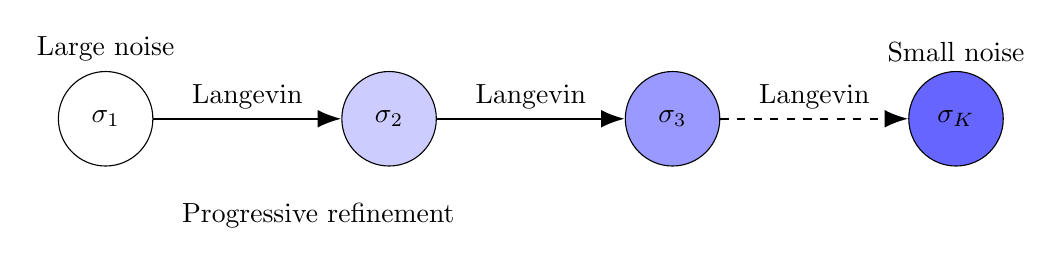
\begin{tikzpicture}[scale=0.9]
  % Noise levels
  \foreach \i/\label in {0/$\sigma_1$,2/$\sigma_2$,4/$\sigma_3$,6/$\sigma_K$}{
    \node[draw, circle, minimum size=1.2cm, fill=blue!\i0!white] (n\i) at (\i*2,0) {\label};
  }
  
  % Arrows
  \draw[-{Latex[length=3mm]}, thick] (n0) -- (n2) 
    node[midway, above] {Langevin};
  \draw[-{Latex[length=3mm]}, thick] (n2) -- (n4) 
    node[midway, above] {Langevin};
  \draw[-{Latex[length=3mm]}, thick, dashed] (n4) -- (n6) 
    node[midway, above] {Langevin};
  
  % Labels
  \node[above] at (n0.north) {Large noise};
  \node[above] at (n6.north) {Small noise};
  \node[below=0.5cm] at (3,-0.5) {Progressive refinement};
\end{tikzpicture}
\caption{Annealed sampling: progressively refine samples across decreasing noise levels, 
using the corresponding conditional score at each stage.}
\end{figure}

\section{Conclusion}

Score matching has emerged as a foundational technique in generative modeling, 
offering a principled alternative to GANs and VAEs. 
Its key advantages include:
\begin{itemize}
\item \textbf{Tractability:} Avoids computing intractable partition functions
\item \textbf{Stability:} Denoising variants provide robust training signals
\item \textbf{Flexibility:} Applicable across modalities and data types
\item \textbf{Theoretical grounding:} Connections to stochastic processes and thermodynamics
\end{itemize}

The progression from basic score matching through denoising, slicing, and noise conditioning 
illustrates how initial theoretical insights evolved to address practical challenges. 
Modern diffusion models inherit these foundations while adding architectural innovations and training techniques.

Future directions include faster sampling, better likelihood estimation, 
application to structured domains (graphs, proteins, PDEs), 
and integration with other learning paradigms like reinforcement learning and active inference.

\appendix

\section{Mathematical Background}

\subsection{Itô's lemma and stochastic calculus}
For $dX_t = \mu_t dt + \sigma_t dW_t$ and smooth $f$:
\begin{equation}
df(X_t) = \left(\frac{\partial f}{\partial t} + \mu_t \frac{\partial f}{\partial x} 
+ \frac{1}{2}\sigma_t^2 \frac{\partial^2 f}{\partial x^2}\right)dt 
+ \sigma_t \frac{\partial f}{\partial x} dW_t
\end{equation}

\subsection{Fokker-Planck equation}
The density $p_t(x)$ of $X_t$ evolves according to:
\begin{equation}
\frac{\partial p_t}{\partial t} 
= -\nabla \cdot (f(x,t) p_t) + \frac{1}{2}\text{tr}(\nabla\nabla^\top (g(t)^2 p_t))
\end{equation}

\subsection{Stein's identity}
For $x \sim \mathcal{N}(\mu, \Sigma)$ and differentiable $h$:
\begin{equation}
\mathbb{E}[\nabla h(x)] = \mathbb{E}[h(x) \Sigma^{-1}(x - \mu)]
\end{equation}
This underlies score matching for Gaussian distributions.

\section{Implementation Details}

\subsection{Complete training script structure}
\begin{lstlisting}[style=py,caption={Recommended project structure}]
import torch
import torch.nn as nn
import torch.optim as optim
import numpy as np

# Data preparation
def make_swiss_roll(n_samples=1000):
    t = 1.5 * np.pi * (1 + 2 * np.random.rand(n_samples))
    x = t * np.cos(t)
    y = t * np.sin(t)
    return np.stack([x, y], axis=1).astype(np.float32)

# Model (as defined earlier)
# Training functions (as defined earlier)

# Main training loop
if __name__ == "__main__":
    data = make_swiss_roll(n_samples=2000)
    dataset = torch.tensor(data)
    
    model = ConditionalScoreNetwork(num_classes=10)
    optimizer = optim.Adam(model.parameters(), lr=1e-3)
    
    for epoch in range(100):
        # Training step
        loss = train_step(model, dataset, optimizer)
        
        # Periodic evaluation
        if epoch % 10 == 0:
            samples = sample_langevin_annealed(model, ...)
            evaluate_and_visualize(samples, data)
\end{lstlisting}

\section*{Acknowledgments}
These notes synthesize ideas from Aapo Hyv\"arinen, Pascal Vincent, Yang Song, Stefano Ermon, 
Jonathan Ho, Jascha Sohl-Dickstein, and many others who developed score-based generative modeling. 
The Python implementations build on publicly available codebases and are intended for educational purposes.

\bibliographystyle{plain}
\begin{thebibliography}{10}

\bibitem{hyvarinen2005}
Aapo Hyv\"arinen.
\newblock Estimation of non-normalized statistical models by score matching.
\newblock \emph{JMLR}, 2005.

\bibitem{vincent2011}
Pascal Vincent.
\newblock A connection between score matching and denoising autoencoders.
\newblock \emph{Neural Computation}, 2011.

\bibitem{song2019}
Yang Song and Stefano Ermon.
\newblock Generative modeling by estimating gradients of the data distribution.
\newblock \emph{NeurIPS}, 2019.

\bibitem{song2020}
Yang Song, Jascha Sohl-Dickstein, Diederik P. Kingma, Abhishek Kumar, Stefano Ermon, and Ben Poole.
\newblock Score-based generative modeling through stochastic differential equations.
\newblock \emph{ICLR}, 2021.

\bibitem{sohl2015}
Jascha Sohl-Dickstein, Eric Weiss, Niru Maheswaranathan, and Surya Ganguli.
\newblock Deep unsupervised learning using nonequilibrium thermodynamics.
\newblock \emph{ICML}, 2015.

\bibitem{ho2020}
Jonathan Ho, Ajay Jain, and Pieter Abbeel.
\newblock Denoising diffusion probabilistic models.
\newblock \emph{NeurIPS}, 2020.

\bibitem{chen2020wavegrad}
Nanxin Chen, Yu Zhang, Heiga Zen, Ron J. Weiss, Mohammad Norouzi, and William Chan.
\newblock WaveGrad: Estimating gradients for waveform generation.
\newblock \emph{ICLR}, 2021.

\bibitem{anderson1982}
Brian D.O. Anderson.
\newblock Reverse-time diffusion equation models.
\newblock \emph{Stochastic Processes and their Applications}, 1982.

\end{thebibliography}

\end{document}
